\newpage
\section{Data aggregation}
\label{aggregation}
\begin{figure}[H]
	\centering
    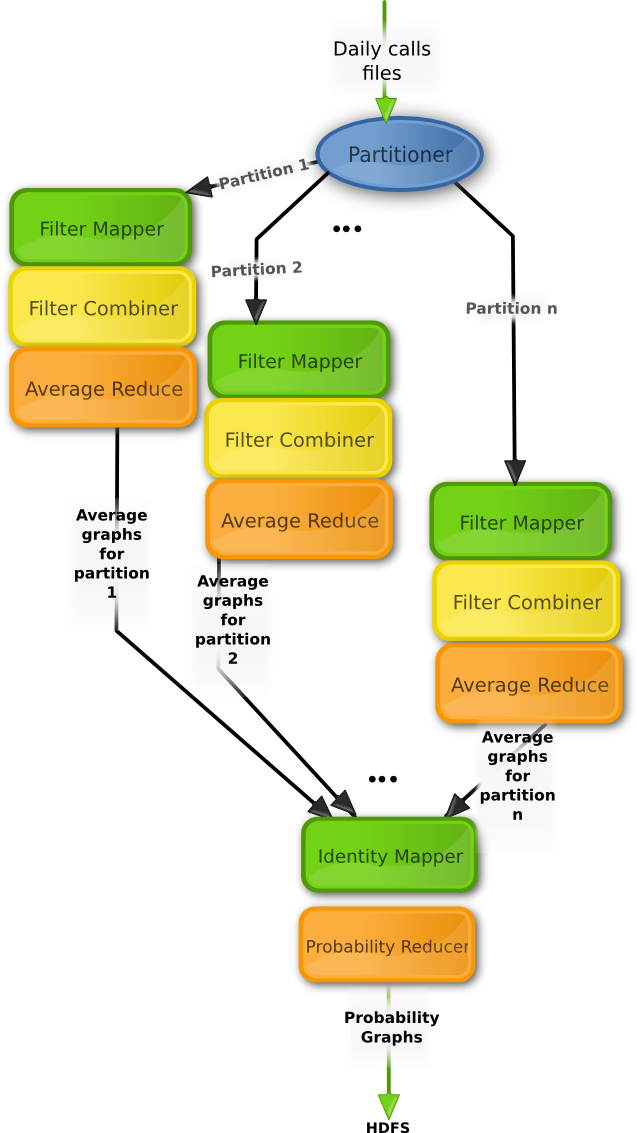
\includegraphics[scale=0.6]{aggregated.png}
    \caption{Driver of the file performing the aggregation task in our work. As it is possible to see, on top
    a partitioner divides in subsequent sequential processes the aggregation phase, which is then recomposed by the \texttt{Identity Mapper} before the final result is produced by the \texttt{Probability Reducer}.}
    \label{fig:aggregated}
\end{figure}

The aim of this part of the project was to produce aggregated probability graphs as defined in section \ref{AVGPG}.
\\ 
We developed a procedure composed by two consecutive logical map reduce computations executable onto the Hadoop environment; the general scheme of the procedure can be seen in \ref{fig:aggregated} and is deeply explained in the following.
The input of the \emph{Time Aggregation} phase is the original dataset (as described in section \ref{thedataset}), while the output is a graph of probabilities of interaction between zones of the considered area
over a certain period of interest, represented as a list of edges.
\subsection{Average graph calculation}
This logical phase aims to calculate several \emph{average graphs} for a given period of interest.
We define an average graph as the graph in which the weight of every arc is the average of the detected strength in input. When no strength is detected in a given 10 minute period, the strength connecting the two areas is considered to be zero. Zero-valued
edges are simply not stored since they would not affect the rest of the computation.
This phase is composed of a map-reduce job, whose pseudo code can be seen in Fig. \ref{fig:filtermap} and Fig. \ref{fig:averagereduce} respectively.
\begin{figure}[H]
\begin{verbatim}
FilterMap(key, value):
// input takes in input all dataset files
// key is bytes read, value is (timestamp,sourceNode,destNode,strength)
// implementeted in aggregated_graphs.FilterMapper.java
    for(i in configuration.all_periods):
        if (value.timestamp belongs_to i):
  	        k = (i.id,i.num,d.sourceNode,d.destNode)
  	        v = value.strength
            emit(k, v)

\end{verbatim}
\caption{Filter Map pseudo-code. Every row of the initial timestamp is checked against the periods of interest defined
as parameter of the computation configuration.all\_periods to understand if it belongs to it. In such case, it
is emitted labeled with the identifier of the aggregation and the number of 10 minutes slots in the whole aggregation.}
\label{fig:filtermap}
\end{figure}
The mapper filters only the interesting entries in the dataset, and labels them with an appropriate identifier for the aggregation. The output key is composed by the  a triple \texttt{(AggregationId,SourceId,DestId)} while the key is the strength value.\\
In the reducer, we calculate the sum of all such values and then divide it by the number of ten minutes slots in the aggregation.
\begin{figure}[H]
\begin{verbatim}
AverageReduce(key,values):
// key is (aggregationId,aggregationLength,sourceNode,destNode), 
// values are strengths
// implemented in aggregated_graphs.AverageReducer.java
    sum = 0
    for v in values:
        sum += v
        (id,num,source,dest) = parse(key)
        avg = sum / num
        emit((id,source),(dest,avg))
\end{verbatim}
\caption{Average Reduce pseudo-code. Calculates for every aggregation period the average stength of connection between any pair of nodes.}
\label{fig:averagereduce}
\end{figure} 
\subsubsection{Implementation details}
During the initial executions, our testing environment
could not successfully compute aggregations over huge periods, because of \textbf{lack of free disk space}. \\
The problem was due to the fact that, in the first map, even though the filter would reduce in general the size of the input data,
this reduction was not enough to fit disks on certain nodes of the cluster before going on with the conseguent reduce phase.\\
With a worst case calculation, in fact, an input split containing all nodes in a graph would produce a graph containing $100.000.000$ of arcs, each one with a weight which could be approximated to 24 Bytes, thus achieving approximately an output of $~$ 2GB. \\
To cope with this issue, we went through a number of different approaches, to finally discover that a \emph{"classic"} splitting technique, along with the benefits provided by the combiner, would result in the best solution for our environment.
\begin{enumerate}
\item \textbf{Combiners} a combiner has been defined to shrink the first map output size. The combiner performs a sum over all strengths in the same aggregation period and, of course, with same source and destination. 
The output of the combiner is a graph for each aggregation period in which the strength is the sum of all strength.

This solution, for an aggregation with containing $n$ 10 minutes slots, could reduce the output of each map task up to $1/n$ of the original size without the combiner. 
The pseudo-code of the combiner used is depicted below:
\begin{verbatim}
FilterCombine(key, values):
//key is (aggregation.id,aggregation.num,sourceNode,destNode)
//values is the list of strengths 
//of the aggregation for the couple (sourceNode, destNode)
    sum = 0
    for v in values:
        sum += v
    context.write(key, sum)
\end{verbatim}
\item \textbf{GZip} another approach that we tried, and thereafter discarded, was to use GZip as compression codec for data going out of the map. From experimental results, we noticed that this approach, altough not providing enough benefits
to cope with disk utilization issues, slowed down our computation significantly.
\item \textbf{Change in split size} thanks to the combiner, the biggest is the number of time slots gathered in a single aggregation, the biggest is the shrinking in data. 
Therefore, we tried to increase the size of the splits to be given to a single map task to exploit this reduction. We progressively increased split size from 128MB to 1GB and then to contain a single whole file, which was defined as not splittable.
However, we noticed that this method, while decreasing the efficiency in the cluster utilization (as only fewer processing units could be used together) and in the completion time of this phase, was still not enough to cope with our disk issues.
\item \textbf{Divide and conquer} the latest, and best approach to solve the disk space issue, was to change the logic in the driver so that what was previously the first map-reduce phase, has been decomposed into several little map-reduce phases, each one taking a parametric number of files of the dataset.
This partitioning method, in which a partition is processed in parallel and the next partition can be processed only when the previous aggregated graphs have been written on HDFS, can be indeed seen as a generalization of the previous case, but allowing to compute what we called \emph{average graphs} even in a space constrained environment. 
Sadly, the introduction of this "partitioning" has some drawbacks, since it will make necessary to introduce a sorting phase in the probability reducer, necessary to eliminate duplicates.
\item \textbf{Other attempts} we also went through several other ways, among which the decommissioning of the nodes (node 0, node 1 and node 2) with less space, trying to avoid to fill the disk completely.
However, this solution (even impreved using the hadoop balancer) was very slow and, as obvious, led to a severe cluster underutilization that we didn't consider acceptable.
\end{enumerate}
We finally adopted a solution in which the split size has been set to 512MB to exploit better the combiner, only a partition of files is processed in parallel (to avoid balancing with 62 files we chose the size of the partition to be 11 files) and a combiner is used in the first phase to reduce both disk and network bandwidth utilization.
Counterintuitively, the sequentialization performed with this approach, with an appropriate partition size allowing to exploit fully the parallelism degree of the environment, when operating with huge datasets led to benefits also in terms of completion time. 
With smaller inputs, however, there's a degradation in terms of completion time (as shown in \ref{fig:partitioningtimes}), even though it is not drammatic.

\begin{figure}[H]
\centering
\begin{tabular}{| c | c | r |}
\hline
\textbf{Partition size} & \textbf{Execution time} \\
\hline
1 File & 2h 20' 45'' \\
\hline
5 Files &  1h 11' 38''\\
\hline
9 Files & 1h 06' 2'' \\
\hline
\end{tabular}
\caption{Execution times for generating the average probability graphs with different partition sizes over (about) 56GB of data in 9 files. All of these computation have been performed with 10 reducers.}
\label{fig:partitioningtimes}
\end{figure}

Our hypothesis is that, after a certain (cluster-dependant) threshold in the size of data is met, the I/O and network bottleneck do not allow to grow in speed, while the huge number of tasks contending the resources would result in a severe slowdown.


The choice of the number of reducers deserves an explanation.
We choosed to perform all the benchmarks above using 10 reducers. 

This number has been chosen for several reasons:
\begin{itemize}
\item It reduces data movement
\item It reduces the completion time, by exploiting better the disks and the processors
\item It allows, in case of failure, to perform the reduce again on a smaller amount of data with respect to the case with just one reducer
\item The size of partitions produced by each mapper task will in general be reduced, allowing to use less disk space.
\end{itemize}

By experimental results, we noticed that the completion time decreased by incrementing the number of reducers up to 10, were substantially the same between 10 and 15, while with more than 15 reducers a small degradation could be observer. 

Finally, the whole dataset aggregations have been performed with 12 reducers, this number seeming a suitable one because of the number of nodes (6) in our architecture. 

\subsection{Probability graph calculation}
The probability graph calculation follows immediately the phase of average graph calculation.\\
In this phase we calculate a probability graph in which an arc represents the probability of transition between the two nodes that it connects. 
This is an average probability in our specific case, since it is achieved receiving as input an average graph.
Also this phase is composed of a map-reduce job, whose pseudo code is shown in \ref{fig:identitymap} and \ref{fig:probabilityreduce}.

The map is a mere identity, while the reduce calculates the total weight of the arcs belonging to the forward star of a single node, to then rescale in terms of probabilities every arc.
  
\begin{figure}[H]
\begin{verbatim}
IdentityMap(key, value):
//key is aggregation.id, sourceNode
//value is destNode, averageStrength
    emit(key, value)
\end{verbatim}
\caption{Identity Map pseudo code. In this case the key is the aggregation identifier and the source node, while the value is a couple destination, average strength}
\label{fig:identitymap}
\end{figure}
\begin{figure}[H]
\begin{verbatim}
ProbabilityReduce(key, values):
	//Key is aggregation.id, sourceNode
	//values is a list of couples in the form (destinationNode, averageStrength)
    sum = 0
    a_list = []
    for v in values:
        (dest, weight) = parse(v)
        sum += weight
        a_list.append((dest,weight))
  
    for a in a_list:
        emit((key.src, a.dest), a.weight / sum)

\end{verbatim}
\caption{Probability Reduce pseudo code.}
\label{fig:probabilityreduce}
\end{figure}
\subsection{Driver}
The driver module - the one which creates and lanches the Hadoop
map and reduce jobs - takes the following input parameters:
\begin{enumerate}
\item \textbf{Aggregation file}, the file containing the descriptions of the aggregations to be performed
\item \textbf{Input directory}, the directory containing the files with the daily calls measurements
\item \textbf{Output directory}, the directory in which the average probability graph will be written
\item \textbf{Partition size} in terms of files per partition. The default is 1. To take the whole dataset must be 0.
\item \textbf{Number of reducers}, by default corresponds to the number of aggregations to perform.
\end{enumerate}
The driver reads the aggregation file, and then saves the aggregation representation in the context, in order for it to be accessible to map and reduce tasks in the first phase.\\
Then there's an iteration in the files placed inside the input directory, adding files one by one until the size of the partition is met.
Then a single job is executed, calculating the average graph for the given partition before a new partition is calculated and a new average graph calculation starts. \\
Finally, when average graphs have been calculated for each partition, the second part takes all these files in input and proceeds to write in the output directory the average probability graph.
A sketch depicting the driver logic in a dataflow fashion can be found in Fig. \ref{fig:aggregated};
The driver is implemented in the file named 
\href{https://github.com/michele-carignani/hadoop-markov-clustering/blob/master/src/aggregation/TimeAggregatedGraphs.java}{TimeAggregatedGraphs}.

\newpage